\documentclass[oneside,senior,etd]{BYUPhys}

\usepackage[utf8]{inputenc}
\usepackage{rotating} 

\usepackage[russian]{babel}
\usepackage{amsfonts} % Пакеты для математических символов и теорем
\usepackage{amstext}
\usepackage{amssymb}
\usepackage{amsthm}
\usepackage{graphicx} % Пакеты для вставки графики
\graphicspath{{pictures/}}
\usepackage{subfig}
\usepackage{color}
\usepackage[unicode]{hyperref}
\usepackage[nottoc]{tocbibind} % Для того, чтобы список литературы отображался в оглавлении
\usepackage{algorithmic} % Для записи алгоритмов в псевдокоде
\usepackage{algorithm}
\usepackage{verbatim} % Для вставок заранее подготовленного текста в режиме as-is
\usepackage{vmargin}
\setmarginsrb{2cm}{2cm}{2cm}{2cm}{0pt}{0mm}{0pt}{13mm}

\Chair{Кафедра Системного Программирования}
\Lab{~}
\Year{2015}
  \Month{Май}
  \City{Москва}
  \AuthorText{Выполнил}
  \Author{Зинченко Дмитрий Александрович}
  \AuthorEng{Zinchenko Dmitrii}
  \AcadGroup{428}

  \TitleTop{Методы и инструменты разметки требований}
  \TitleBottom{в многоверсионных текстовых документах} % leave empty if you don't need it
  \TitleTopEng{Methods and instruments of requirement marking up}
  \TitleBottomEng{in multiversion documents} % leave empty if you don't need it
  
 \docname{Выпускная квалификационная работа}
  \Advisor{Хорошилов Алексей Владимирович}
  \AdvisorDegree{к.ф-м.н.\\}
  


\Abstract{В данной работе исследуется и проектируется алгоритм поиска соответствий фрагментов текста, выделенных в старой версии документа, фрагментам новой версии того же документа. Проводится оценка работы алгоритма на тестовой базе и сравнение с существующим алгоритмом, использующимся в системе управления требованиями Requality}
\AbstractEng{In this work, algorithm of matching text fragments from the old version of the document to the fragments of the new version of the same document is designed. The algorithm is tested on document base and compared to existing method used in requirement management system Requality}


%%%% DON'T change this. It is here because .sty does not support cyrillic cp properly %%%%
\University{Московский Государственный Университет имени М.В.Ломоносова}
\Faculty{Факультет Вычислительной Математики и Кибернетики}
\GrText{студент группы}
\AdvisorText{Научный руководитель}
\AbstractText{Аннотация}

\begin{document}
\fixmargins
 \makepreliminarypages

\oneandhalfspace

\tableofcontents

\section{Введение}
\label{sec:Chapter1} \index{Chapter1}
Выявление и отслеживание требований является важной частью проектирования программных систем, при этом отслеживание выполнения требований остается важным на протяжении всего жизненного цикла системы. Подробнее процессы разработки программного обеспечения описываются в \cite{web:DevelopmentProcesses}. На рисунке \ref{intro:image1} в качестве примера показан цикл итеративной разработки системы.

\begin{figure}[h]
\begin{center}
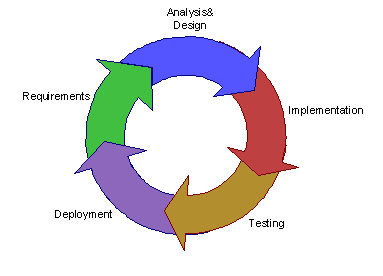
\includegraphics[scale=0.85]{SoftwareDevelopment.png}
\caption{\emph{Диаграмма цикла итеративной разработки программной системы}}
\label{intro:image1}
\end{center}
\end{figure}

В дальнейшем под понятием требование мы будем понимать утверждение относительно свойств и атрибутов, которыми должна обладать программная система, чтобы удовлетворять стандартам, спецификациям или другим формальным документам. \cite{book:Requirements} \cite{book:SWEBOK}

В процессе разработки ПО важно отслеживать, удовлетворяет ли текущая версия системы требованиям, описанным в спецификации, проверяют ли написанные тесты все требования, которым должен удовлетворять продукт, и уточнять требования на каждой итерации разработки. Для этих целей служат системы управления требованиями, одной из которых является Requality \cite{web:Requality}, разрабатываемая в Институте Системного Программирования РАН.

Совокупность требований к программной системе представляет собой некоторую иерархическую структуру - каталог требований. Некоторые системы управления требованиями позволяют хранить связанные с требованиями версии спецификаций и отслеживать связь между фрагментами текста спецификации и требованиями. Таким образом, каждому требованию соответствует один или несколько выделенных специальным образом участков текста спецификации требований. При обновлении спецификации возникает потребность в изменении каталога требований и поиске в новом тексте фрагментов, соответствующих требованиям. Этот функционал становится особенно полезным при работе со стандартами, новые версии которых разрабатываются независимо от команд, их использующих.

Поскольку часто бывает так, что новая версия спецификации требований отличается от предыдущей незначительно, и текст большей части требований в двух версиях документа совпадает, задача переноса выделения текста тех требований, которые остались без изменений, в новую версию документа, становится актуальной. Автоматизация решения этой задачи упрощает и ускоряет выделение требований в новой версии спецификации требований. Исследованию задачи переноса требований между версиями документа и посвящена эта работа.

\subsection{Используемая терминология}
Для проектирования разрабатываемой системы и постановки задачи введем следующие понятия:
\begin{itemize}
\item \textbf{Документ} – текстовый файл, являющийся синтаксически корректным XHTML документом.
\item \textbf{Теги требования} (в рамках системы Requality)– пара тегов

\emph{<span class=”requality\_text id\_***”> 	</span>},

где *** - идентификационный номер требования. Помимо этого, в Requality после открывающего тега требования и перед текстом внутри него, может находиться пара тегов 

\emph{<a name="***" id="***" class=”requality\_id”></a>},

позволяющая интерфейсу системы определять, на каком фрагменте текста центрировать редактор документов при выборе требования. Под \textbf{разметкой требований} будем понимать совокупность тегов требований в документе.

\item \textbf{Фрагмент требования} – участок документа, ограниченный тегами требования. Фрагмент не может содержать XHTML теги внутри себя.

\item \textbf{Объединение фрагментов требования} – несколько фрагментов одного и того же требования, идущих подряд.

Пример выделенных в инструменте Requality фрагментов требований и xhtml тегов, ограничивающих их, продемонстрирован на рисунках \ref{intro:image2} и \ref{intro:image3} соответственно.

\begin{figure}[h]
\begin{center}
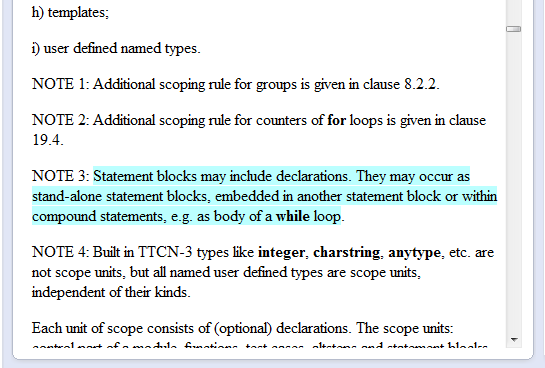
\includegraphics[scale=0.8]{requirement.png}
\caption{\emph{Пример объединения фрагментов требований в системе Requality}}
\label{intro:image2}
\end{center}
\end{figure}

\begin{figure}[h]
\begin{center}
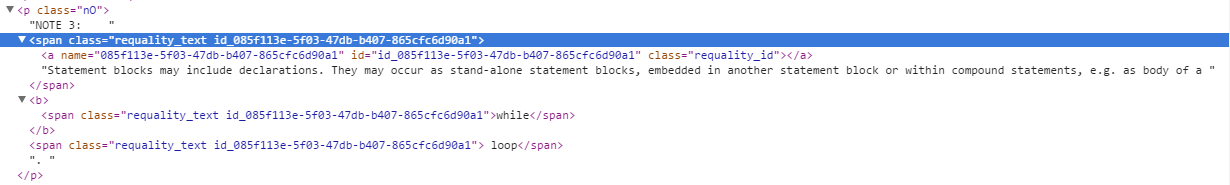
\includegraphics[scale=0.55]{tags.png}
\caption{\emph{Структура xhtml тегов для выделенных фрагментов}}
\label{intro:image3}
\end{center}
\end{figure}

\item \textbf{Требование} (в рамках системы Requality)– логическое объединение фрагментов текста, ограниченных тегами требований с одинаковыми идентификационными номерами. \textbf{Идентификационный номер требования} – номер, использующийся в тегах требования, соответствующих ему. Идентификационный номер требования уникален, двух разных требований с одним номером не существует.

\item \textbf{Исходный документ} – документ, представляющий рабочую версиию некоторой спецификации, может содержать разметку требований. Неформально - документ, разметка требований которого определена, и которую необходимо перенести.

\item \textbf{Конечный документ} – документ, для которого разметка требований не определена. В общем случае конечный документ может быть никак не связан с исходным, однако тогда задача переноса разметки требований между версиями документа становится бессмысленной. Конечный документ представляет собой новую версию спецификации, в которую требуется перенести требования.

\item Часть конечного документа считается \textbf{полностью соответствуещей} объединению фрагментов текста исходного документа, если содержимое объединения фрагментов текста исходного документа совпадает с частью конечного документа с точностью до незначащих символов и тегов XHTML. В противном случае часть конечного документа \textbf{не соответствует} содержимому объединения фрагментов исходного документа.

\item Под \textbf{переносом объединения фрагментов требования} мы будем понимать перенос тегов требования, ограничивающих все фрагменты этого объединения, из исходного документа в конечный. 

\item Под \textbf{переносом требования} мы будем понимать перенос всех его объединений фрагментов, для которых в конечном документе было найдено полное соответствие. 

\item \textbf{Незначащие символы} - пробелы, переносы строк и знаки препинания.

\item \textbf{Структурная разметка документа} – xhtml теги заголовков и абзацев (теги \emph{<h1> --- <h6>, <p>, <blockquote>})

\end{itemize} % Введение
\section{Постановка задачи}
\label{sec:Chapter2} \index{Chapter2}
В рамках выпускной квалификационной работы необходимо разработать библиотеку, позволяющую осуществлять перенос требований из исходного документа в конечный.

Стоит отметить, что в поставленной задаче считается, что оба документа имеют схожую структурную разметку и названия подразделов, в которых находятся фрагменты требований. Перенос объединений фрагментов требований, для которых не найдено точного соответствия, выходит за рамки данной работы, хотя и может быть осуществлен путем построения функции схожести фрагментов текстов.
 % Постановка задачи
\section{Проектирование системы}
\label{sec:Chapter3} \index{Chapter3}
\subsection{Возможные сценарии использования библиотеки}
\begin{itemize}
\item \textbf{Получение объектной модели документа}

Согласно \cite{book:DOM}, \cite{book:JDOM}, \textbf{Объектная модель документа} (Document Object Model – DOM) – стандарт, предложенный веб-консорциумом, и регламентирующий способ представления содержимого документа (в частности – xhtml документа) в виде набора объектов. DOM позволяет представить любой документ в виде иерархической структуры (дерева) узлов, каждый из которых соответствует элементу, атрибуту, текстовому, графическому или любому другому объекту.

Одним из инструментов, позволяющих извлекать DOM модель документа из текстового файла, является библиотека JDOM (в данной работе используется версия 2.0.6).
По имени файла исходного документа осуществляется получение структуры данных (дерева), соответствующего объектной модели документа. Схематичный пример полученного из документа DOM дерева изображен на рисунке \ref{pr:image4}.

\begin{figure}[h]
\begin{center}
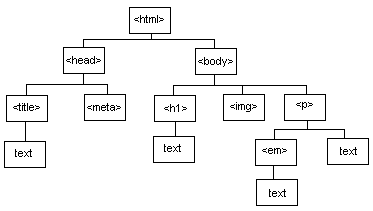
\includegraphics[scale=1.4]{dom.png}
\caption{\emph{Пример DOM модели документа}}
\label{pr:image4}
\end{center}
\end{figure}

\item \textbf{Выделение структурной разметки документа из его DOM дерева}

По DOM модели документа осуществляется построение дерева, отражающего его структурную разметку.

\item \textbf{Получение списка требований по дереву документа}

Выделение фрагментов требований из дерева с дальнейшей группировкой по id. 

Из дерева структурной разметки документа извлекается список требований(объектов), каждое требование содержит идентификационный номер и список фрагментов текста, содержащихся в нем.

\item \textbf{Синхронизация по фрагменту требования}

По фрагменту требования находится вершина дерева разметки исходного документа, в тексте которой содержится данный фрагмент.

\item \textbf{Получение пути в дереве разметки от корня до элемента}

По дереву разметки документа осуществляется поиск последовательности вершин – пути в дереве от корня до данной вершины

\item \textbf{Поиск элемента, соответствующего данному, в дереве другого документа}

По элементу дерева разметки одного документа осуществляется поиск элемента разметки другого документа такого, что пути из корней деревьев до элементов имеют одинаковые типы вершин и идентичный (с точностью до незначащих символов) текст.

\item \textbf{Перенос объединения фрагментов требования}

В конечном документе осуществляется поиск участка текста, соответствующего объединению фрагментов требования, и осуществляется перенос тегов фрагментов в найденные позиции (начало и конец найденного участка текста).

\item \textbf{Перенос требования}

Попытка переноса всех фрагментов требования.

\end{itemize}

\subsection{Использование библиотеки JDOM}

Важным этапом работы любого алгоритма, решающего поставленную задачу, является получение и хранение содержимого исходного и конечного документов. Одним из инструментов, позволяющих это сделать, является библиотека JDOM, используя которую можно получить DOM модель по XML документу. Также JDOM позволяет эффективно получить все фрагменты требований из исходного документа.

Помимо этого, JDOM предоставляет средства для редактирования XML документов, что является лучшим способом добавить разметку в конечную версию документа после осуществления переноса  фрагментов требований.

В статье \cite{web:JDOM} описываются возможности и приводятся примеры использования JDOM.

\subsection{Обзор решения, применяемого в Requality}

\subsubsection{Основная идея}

Решение проблемы переноса разметки требований, использующееся на данный момент в Requality, основано на сравнении исходного и конечного документа без XHTML разметки, как строк текста (plain text). Для сравнения используется библиотека google-diff, в качестве результата сравнения двух текстов возвращающая список объектов Diff, каждый из которых содержит описание операции, которую нужно выполнить с текстом исходного документа.

Статья \cite{web:Diff} описывает ключевой алгоритм, использующийся в google-diff.

Операции имеют формат \emph{(<Тип операции>, <Текст>)}, где \emph{Тип операции} - одна из трех команд "EQUAL"\, "DELETE"\, "INSERT"\, а \emph{Текст} - часть текста исходного документа, над которой операцию необходимо совершить. Гарантируется, что при последовательном выполнении операций из списка из текста исходного документа получится текст конечного. Пример результата работы Diff алгоритма изображен на рисунке \ref{pr:image5}.

\begin{figure}[h]
\begin{center}
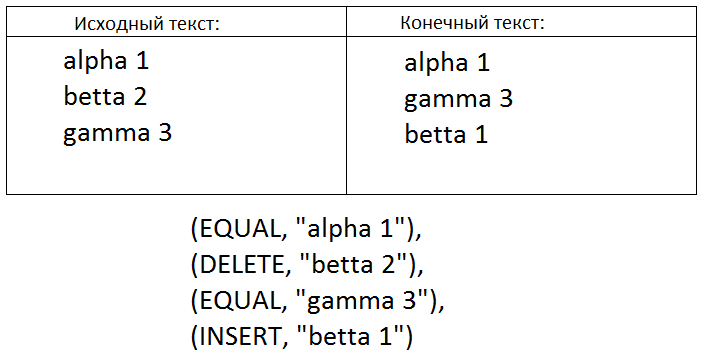
\includegraphics[scale=0.9]{diffResult.png}
\caption{\emph{Пример результата работы diff алгоритма}}
\label{pr:image5}
\end{center}
\end{figure}

\subsubsection{Алгоритм}

Исходный документ преобразуется в DOM дерево, и из него извлекаются все выделенные фрагменты требований, которые нужно перенести. Затем осуществляется преобразование исходного и конечного документа в текстовые данные без XHTML разметки, при этом позиции в исходном тексте извлеченных ранее фрагментов требований запоминаются. Два полученных текста подаются на вход Diff алгоритму, который возвращает список операций, описывающих разницу между исходным и конечным документом.

После окончания работы Diff алгоритма для каждого фрагмента требования из исходного текста определяется, находился ли он в блоке EQUAL результата работа Diff, и если да, то осуществляется перенос соответствующих тегов требования в DOM дерево конечного документа. В противном случае считается, что фрагмент перенести не удалось. Обновленный конечный документ восстанавливается по измененному DOM дереву.

Таким образом, алгоритм можно представить в виде диаграммы, изображенной на рисунке \ref{pr:image6}.

\begin{figure}[h]
\begin{center}
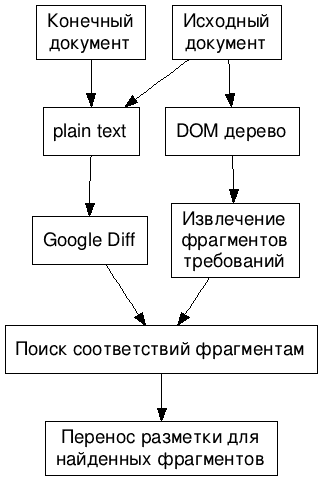
\includegraphics[scale=0.7]{reqSolutionPresentation.png}
\caption{\emph{Диаграмма алгоритма переноса разметки требований системы Requality}}
\label{pr:image6}
\end{center}
\end{figure}

\subsubsection{Характеристики}

Важной особенностью такого подхода к решению задачи является независимость получения результата от разницы между разметкой исходного и конечного документов. Если в новой версии документа была использована разметка, отличная от старого, то это не повлияет на эффективность работы алгоритма, поскольку разметка документов используется только при поиске фрагментов требований. С другой стороны, решение, основанное на использовании diff-алгоритма, перестает работать в случае перестановки разделов в конечном документе, и может работать существенно хуже в случае добавления большого количества новых разделов и текста.

Помимо этого, в текущей реализации этого алгоритма есть фрагменты, соответствие которым находится, однако перенос не осуществляется в связи с различными трудностями работы с DOM моделью документа.

\subsection{Предлагаемое решение}

Основной идеей решения поставленной задачи, которое описывается в данной работе, является локализация места конечного документа, в котором осуществляется поиск соответствия фрагменту, выделенному в исходном документе. В качестве места, в котором нужно осуществлять поиск, в конечном документе выбирается подраздел, соответствующий (в дальнейшем будет описано, как) подразделу исходного документа, содержащего искомый фрагмент требования.

После проведения этой операции размер текста, в котором нужно найти соответствие фрагменту требования, считается достаточно маленьким для применения алгоритма прямого поиска. В том случае, если совпадение с текстом фрагмента было найдено, осуществляется перенос разметки в соответствующее место конечного документа.

\subsection{Внутреннее представление документа}

Однако DOM дерево, полученное из исходного и конечного документов, не удовлетворяет полностью потребностям такого решения - текст раздела в таком дереве не привязан к заголовку, а заголовки, являющиеся вложенными в документе, в DOM дереве находятся на одном уровне иерархии. Таким образом, DOM модель не отражает структурную разметку документа.

Поэтому для удобства работы с иерархией разделов документов было решено осуществлять построение на основе DOM моделей документов деревья, позволяющие проще отслеживать вложенность разделов и связь текстов разделов с их заголовками.

Пример DOM дерева документа, и построенного по нему дерева структурной разметки можно наблюдать на рисунках \ref{ris:DOMtree} и \ref{ris:MYtree} соответственно:

\begin{figure}[h]
\begin{center}
\begin{minipage}[h]{0.55\linewidth}
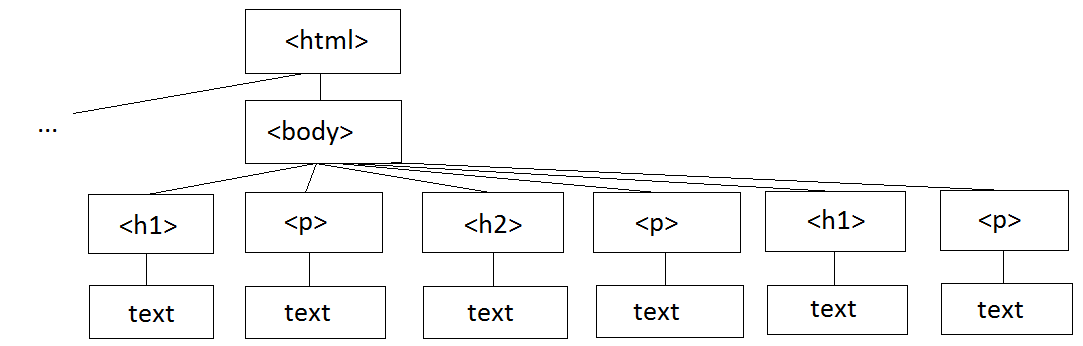
\includegraphics[width=1\linewidth]{good_dom_tree.png}
\caption{\emph{DOM дерево документа.}} %% подпись к рисунку
\label{ris:DOMtree} %% метка рисунка для ссылки на него
\end{minipage}
\hfill 
\begin{minipage}[h]{0.4\linewidth}
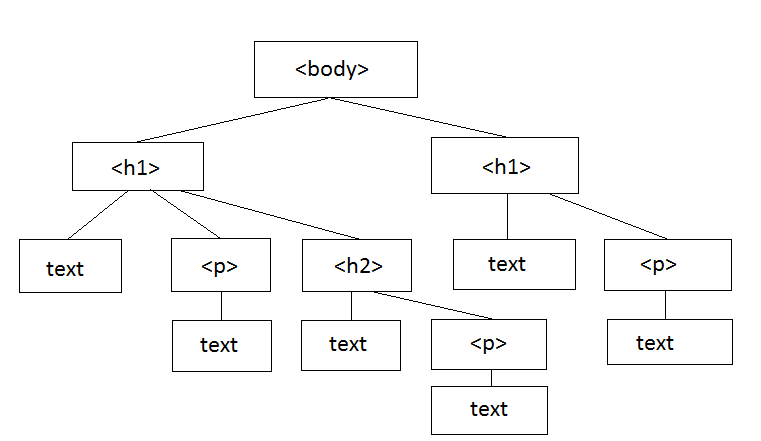
\includegraphics[width=1\linewidth]{my_tree}
\caption{\emph{Построенное дерево структурной разметки.}}
\label{ris:MYtree}
\end{minipage}
\end{center}
\end{figure}

Основываясь на введенном новом представлении документа, определим следующие понятия:

\textbf{Путь до раздела документа} – список вершин в пути в дереве разметки документа до вершины, соответствующей разделу.

\textbf{Путь до фрагмента требования} – путь до вершины дерева разметки максимальной глубины, соответствующей разделу, в котором содержится этот фрагмент.

\subsection{Алгоритм}

Таким образом, алгоритм переноса разметки требований между версиями документа выглядит следующим образом:

\begin{enumerate}
\item Извлечь содержимое исходного и конечного документов при помощи JDOM

\item Построить на основе DOM деревьев документов деревья структурной разметки

\item Извлечь требования из дерева исходного документа

\item Для каждого объединения фрагментов требования:

\begin{enumerate}

\item Получить путь до объединения фрагментов требования

\item Получить по дереву разметки конечного документа путь до соответствующего раздела

\item Найти вхождение текста объединения фрагментов в полученном разделе.

\item Если путь в дереве разметки конечного документа или вхождение текста объединения фрагментов в разделе конечного документа не было найдено, считать, что перенос каждого фрагмента из объединения осуществить не удалось. В противном случае - изменить структуру части дерева разметки, соответствующей разделу конечного документа, добавив в неё фрагменты требования

\item Изменить структуру соответствующей разделу части DOM дерева конечного документа

\end{enumerate}

\item Изменить конечный документ в соответствии с изменением структуры его DOM дерева

\end{enumerate}

\subsection{Характеристики}

В силу особенности построения дерева разметки для исходного и конечного документов, добавление, изменение или удаление разделов, не содержащих фрагментов требований, не влияет на эффективность работы алгоритма. Помимо этого, перестановка разделов в конечном документе так же не влияет на перенос фрагментов. 

Однако изменения заголовков разделов, по которым локализуется место поиска соответствия объединению фрагментов требования, а так же изменения вложенности подразделов, в которых ищутся фрагменты, влияют на перенос разметки в конечный документ - если полное соответствие пути до объединения фрагментов в дереве разметки исходного документа не было найдено, перенос фрагментов не осуществляется.

Помимо этого стоит отметить, что предложенный алгоритм гораздо проще обобщить на случай, когда в конечном документе существует лишь частичное соответствие тексту объединения фрагментов, чем алгоритм, основанный на применении diff. Подробнее об этом будет рассказано в заключении. % Обзор существующих решений
\section{Устройство системы}
\label{sec:Chapter4} \index{Chapter4}

\subsection{Дерево структурной разметки документа}

Каждая вершина дерева структурной разметки имеет следующие поля: тип, текст содержимого и список вершин - сыновей и вершину-родителя. Изначально текст содержимого для вершины не определен, и заполняется в том случае, если в процессе переноса фрагментов требований вызывалась функция получения текста раздела, описанная ниже. Тип вершины дерева не фиксирован и зависит от соответствующей вершины DOM модели. Тремя зафиксированными типами вершин являются: 

\begin{itemize}

\item \textbf{"text"} - в случае если вершина содержит текстовую информацию. Может находиться только в листьях дерева. Если тип вершины - \emph{"text"}, в ней заполняется специальное поле, в котором запоминается содержимое соответствующего вершине участка текста документа.

\item \textbf{"body"} - содержится в единственном экземпляре в корне дерева.

\item \textbf{"requirement"} - в случае, если вершина содержит фрагмент требования. Может иметь только одного потомка типа \emph{"text"}. Если тип вершины - \emph{"requirement"}, в ней заполняются специальные поля, служащие для формирования списка требований и дальнейшего переноса фрагмента во в конечный документ.

Поле id содержит идентификационный номер требования, к которому относится фрагмент, соответствующий вершине. Поле a содержит \emph{true} или \emph{false} в зависимости от того, нужно ли добавлять пару тегов ссылки на требование \newline(\emph{<a name="***" id="***" class=”requality\_id”></a>}) после переноса фрагмента в конечный документ. 

\end{itemize}

\subsection{Построение дерева структурной разметки по DOM модели документа}

Построение вершин дерева структурной разметки осуществляется в порядке обхода DOM дерева в глубину \cite{book:Programming}. При этом вершины, не влияющие на структуру документа, игнорируются и не участвуют в построении дерева структурной разметки. В данной работе к вершинам, влияющим на структуру документа, вершины DOM модели документа, имеющие имена \emph{"span"\, "a" (в случае, когда вершина с именем "a" является потомком вершины, соответствующей фрагменту требования)\, "h1---h6"\, "p"\, и "blockquote"}. Соответствующая вершина дерева структурной разметки создается на основе текущей рассматриваемой вершины DOM модели.

Для организации иерархии параграфов и разделов используется стек (эта структура данных подробно описана в \cite{book:Programming}): При прохождении в DOM дереве вершины заголовка раздела проверяется, есть ли такой тип раздела в стеке. Если его нет, то считается, что текущий раздел является подразделом последнего встреченного раздела и соответствующая ему вершина добавляется в стек. В противном случае из стека извлекаются вершины дерева до тех пор, пока извлеченная вершина не будет иметь тот же тип, что и добавляемая, а затем родителем добавляемой вершины становится родитель извлеченной из стека. Таким образом вершины подразделов одного и того же раздела в дереве структурной разметки имеют одинаковую глубину.

В случае, если текущая рассматриваемая вершина DOM модели документа имеет имя \emph{span} и атрибут \emph{class}, начинающийся с \emph{"requality\_text"}, в дереве разметки создается вершина, имеющая тип requirement, и в ней заполняются поля \emph{id} и \emph{a}. По умолчанию считается, что такие вершины содержатся только в исходном документе.

\subsection{Устройство требования}

\begin{itemize}
\item \textbf{Фрагмент требования (Location)}

Объект этого типа содержит ссылку на соответствующую фрагменту вершину дерева разметки. Предоставляет метод, позволяющий определять порядковый номер вершины в списке сыновей её родителя.

\item \textbf{Объединение фрагментов (ActualLocation)}

В силу особенностей выделения фрагментов требований в системе Requality, подряд идущие участки текста, соответствующие одному требованию, могут находиться в разных фрагментах из-за наличия разметки. Перед переносом такие участки нужно объединить в один, для которого и должен осуществляться поиск соответствия в конечном документе.

\item \textbf{Требование (Requirement)}

Объект каждого требования содержит \emph{id} требования, список фрагментов, относящихся к нему, и список объединений фрагментов, полученный в результате обработки списка фрагментов. Объединение фрагментов происходит в том случае, если они имеют общего родителя, и их порядковые номера, как сыновей, отличаются на единицу. Помимо этого, объект типа Requirement содержит информацию о том, нужно ли добавлять пару тегов ссылки на требование, при переносе этого фрагмента.  

\end{itemize}

\subsection{Извлечение текста из дерева структурной разметки}

Текстом вершины X дерева структурной разметки будем называть объединение полей text тех вершин дерева, которые имеют тип text и содержатся в поддереве, корнем которого является вершина X.

\begin{enumerate}
\item \textbf{Текст заголовка}

Текстом заголовка считается объединение текстов всех подряд идущих вершин, являющихся прямыми потомками вершины, соответствующей этому заголовку, до первой вершины, соответствующей абзацу. На рисунке \ref{sys:headertext} фрагмента дерева разметки выделены вершины, текст которых участвует в тексте заголовка h1.

\begin{figure}[h]
\begin{center}
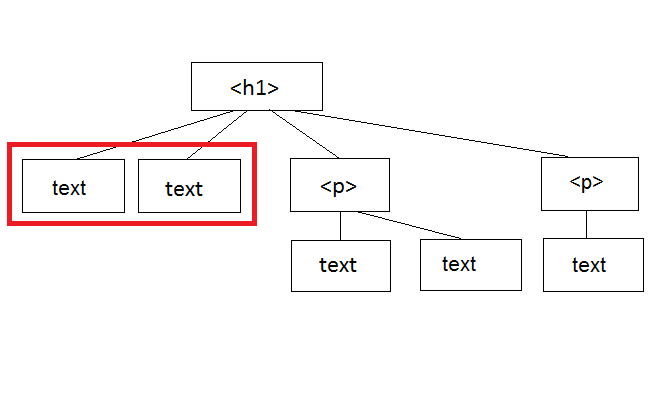
\includegraphics[scale=0.7]{headerText.png}
\caption{Текст заголовка дерева разметки}
\label{sys:headertext}
\end{center}
\end{figure}

\item \textbf{Текст раздела}

Текст раздела содержит в себе текст соответствующего заголовка и текст всех вершин, не являющихся подзаголовками этого раздела. На рисунке \ref{sys:parttext} фрагмента дерева разметки выделены вершины, текст которых включается в текст раздела h1.

\begin{figure}[h]
\begin{center}
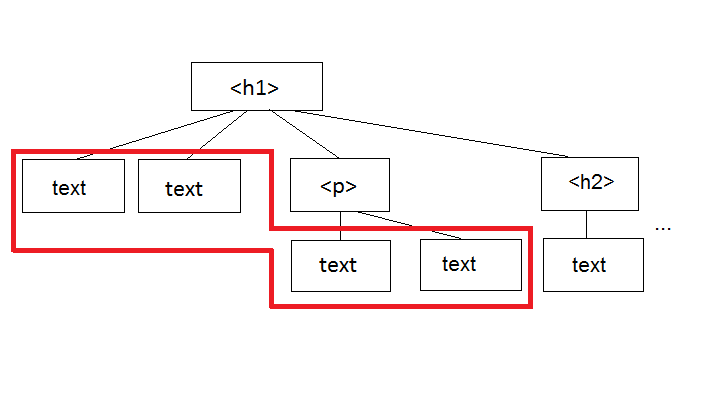
\includegraphics[scale=0.7]{partText.png}
\caption{Текст раздела дерева разметки}
\label{sys:parttext}
\end{center}
\end{figure}

После получения текста раздела он преобразуется при помощи регулярных выражений и запоминается в специальном поле соответствующей вершины дерева структурной разметки документа.

\item \textbf{Использование регулярных выражений}

Поскольку используемые незначащие символы в исходном и конечном документах могут отличаться, для осуществления сравнения и поиска в частях текстов их необходимо привести к унифицированному виду. Для этого используется механизм регулярных выражений, описанный в \cite{book:RegExp}, \cite{web:Reg}. Перед дальнейшим использованием текста раздела или заголовка, над ним осуществляются следующие преобразования:

\begin{itemize}
\item Все пробельные символы заменяются на пробел (символ ' ' в Java)

\item Удаляются все пробельные символы и переводы строк(whitespace characters) в начале и конце обрабатываемой строки

\item Несколько пробельных символов или переводов строк, идущих подряд, заменяются на один.

\item Пробельные символы, идущие перед знаками препинания, удаляются. После знаков препинания добавляется один пробел, если его нет.

\item Перед открывающими скобками добавляется один пробел, если его нет.

\item После открывающих и перед закрывающими скобками удаляется пробел, если он есть.
\end{itemize}

\end{enumerate}

\subsection{Устройство поиска соответствия объединению фрагментов требований}

По объединению фрагментов требования осуществляется поиск пути в дереве разметки исходного документа до подраздела, содержащего это объединение фрагментов. При этом из множества найденных путей выбирается тот, который имеет максимально возможную длину. Путь хранится в виде последовательности указателей на вершины дерева, начиная от корня. 

В дереве разметки конечного документа осуществляется поиск соответствующего пути. Путь B считается соответствующим пути A, если тексты всех заголовков в пути B совпадают с точностью до незначащих символов и цифр с текстами соответствующих заголовков в пути A. В случае если такой путь был найден, считается, что соответствие объединению фрагментов должно находиться в конечном документе в тексте подраздела, соответствующего последней вершине (вершине наибольшей глубины) найденного пути. В противном случае каждый фрагмент из этого объединения считается не перенесенным, и процесс переноса для данного объединения фрагментов требования останавливается.

Если в конечном документе путь, соответствующий пути до объединения фрагментов требования в исходном документе, был найден, то текст соответствующего подраздела конечного документа извлекается, преобразуется с использованием регулярных выражений, и в нём осуществляется поиск текста объединения фрагментов методом прямого поиска \cite{web:StrSearch}. Результатом поиска является позиция (номер символа), где в обработанном тексте подраздела начинается участок текста, полностью совпадающий с текстом объединения фрагментов требования, либо -1, если такая позиция не была найдена. По этой позиции далее осуществляется добавление тегов требований в конечный документ и элементов в соответствующее ему дерево разметки.

\subsection{Добавление элементов требований в дерево разметки документа}

В общем случае найденное соответствие объединению фрагментов лежит в нескольких вершинах дерева разметки конечного документа типа \emph{"text"}. Это объясняется тем, что вершины типа \emph{"text"}, идущие подряд, не объединяются при построении дерева разметки документа, при этом элементы DOM модели документа, не отвечающие за разметку, в построении дерева не используется. В ходе обхода поддерева, соответствующего найденному подразделу, возможны следующие варианты взаимного расположения найденного соответствия объединению фрагментов и вершин типа \emph{"text"}, и соответствующие проводимые операции:

\begin{enumerate}

\item Текст вершины дерева разметки не пересекается с найденным соответствием (находится до номера символа, с которого соответствие объединению фрагментов было найдено). В этом случае текст текущей рассматриваемой вершины пропускается.

\item Текст вершины дерева разметки полностью содержит в себе текст, соответствующий объединению фрагментов.

В этом случае осуществляется разбиение рассматриваемой текстовой вершины на три части (в общем случае, в частных случаях одна или обе пограничных текстовых вершины могут отсутствовать), согласно рисунку \ref{sys:add}, добавляется вершина требования (тип “requirement”) с соответствующим \emph{id}. Процесс преобразования дерева разметки для данного объединения фрагментов после проведения этой операции считается завершенным.

\begin{figure}[h]
\begin{center}
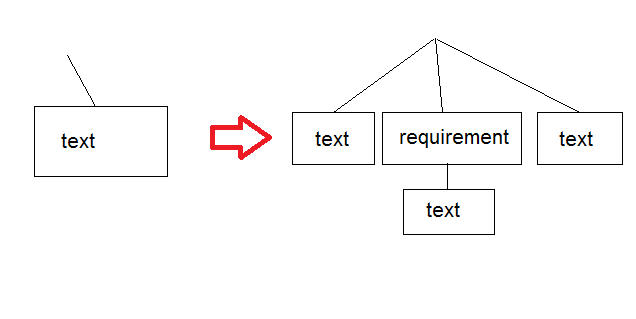
\includegraphics[scale=0.7]{add.png}
\caption{Случай полного вхождения текста объединения фрагметов в текстовую вершину дерева разметки}
\label{sys:add}
\end{center}
\end{figure}

\item Текст вершины дерева разметки частично содержит в себе текст, соответствующий объединению фрагментов. 

В этом случае осуществляется разбиение рассматриваемой текстовой вершины на две части (в общем случае, в частном случае одна пограничная текстовая вершина может отсутствовать) согласно рисунку \ref{sys:addNew}, добавляется вершина требования с соответствующим id. Затем часть текста, для которой была создана вершина типа requirement, удаляется из текста, соответствующего объединению фрагментов требования, и процесс продолжается для последующих текстовых вершин.

\begin{figure}[h]
\begin{center}
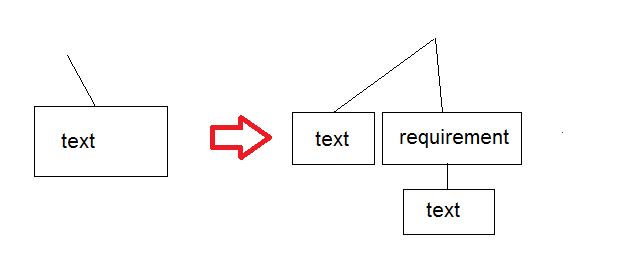
\includegraphics[scale=0.7]{addNew.png}
\caption{Случай неполного вхождения текста объединения фрагметов в текстовую вершину дерева разметки}
\label{sys:addNew}
\end{center}
\end{figure}

\end{enumerate}

\subsection{Добавление разметки требований в DOM модель}

По измененному дереву разметки конечного документа и его DOM дереву синхронно осуществляется обход в глубину - на каждом шаге обхода текущая рассматриваемая вершина дерева разметки соответствует вершине DOM дерева. В случае если рассматриваемая вершина дерева разметки и соответствующая ей вершина DOM дерева имеют тип \emph{"text"}, осуществляется проверка на совпадение содержимого текущих вершин DOM модели и дерева разметки. Если они не совпадают, считается, что эта вершина была изменена в дереве разметки конечного документа из-за добавления элементов требований, и вершину DOM дерева нужно разбить \cite{book:JDOM} на несколько таким же образом, как было описано в предыдущем пункте. Вершина типа \emph{"requirement"} дерева разметки при этом заменяется на вершину DOM дерева с именем \emph{span} и атрибутами \emph{class}, начинающимся \emph{"requality\_text"},  

Поскольку на данном этапе вершины дерева разметки и DOM дерева, тип которых отличен от \emph{"text"}, не влияют на работу этой части программы, их рассмотрение можно опустить, реализовав функции, получающие следующие в порядке обхода дерева в глубину вершины типа \emph{"text"} по текущим в дереве разметки и DOM дереве соответственно. 

После изменения DOM модели конечного документа по ней создается его измененная версия, содержащая теги перенесенных требований.  % Исследование и построение решения задачи
\section{Полученные результаты}
\label{sec:Chapter5} \index{Chapter5}

Описанный ранее алгоритм был реализован на языке программирования Java, и работа реализации была проверена на наборе документов ETSI (\cite{web:etsi461}), IEEE (\cite{web:POSIX2004}, \cite{web:POSIX2008}) и Linux Foundation (\cite{web:LSB3}, \cite{web:LSB4}). Результаты экспериментов приведены в таблице \ref{tabular:results}.

\begin{table}[H]
\caption{Результаты работы предложенного алгоритма на некоторых документах}
\label{tabular:results}
\begin{center}
\begin{tabular}{|p{0.26\linewidth}|p{0.14\linewidth}|p{0.14\linewidth}|p{0.16\linewidth}|p{0.15\linewidth}|p{0.04\linewidth}|}
\hline
\textbf{Название\newlineдокумента} & \textbf{Номер\newline исходной версии} & \textbf{Номер\newlineконечной\newline версии} & \textbf{Примерный объем (тыс. символов)} & \textbf{Перенесено/\newlineнайдено\newline фрагментов} & \textbf{\%} \\
\hline
ETSI TS 103 097 & 1.1.6 & 1.1.12 & 75 & 191/430 &  44.4\\
\hline
TTCN-3 core language part 3 head 5 & 4.5.1 & 4.6.1 & 32 & 323/335 & 96.4\\
\hline
TTCN-3 core language part 4 head 6 & 4.5.1 & 4.6.1 & 104 & 936/969 & 96.5\\
\hline
TTCN-3 core language part 5 head 7 & 4.5.1 & 4.6.1 & 20 & 138/154 & 89.6\\
\hline
POSIX*, fprintf & Issue 6, 2004 & Issue 7, 2008 & 32 & 721/1014 & 71.1\\
\hline
POSIX, fwprintf & Issue 6, 2004 & Issue 7, 2008 & 23 & 651/954 & 68.2\\
\hline
POSIX, environ(exec) & Issue 6, 2004 & Issue 7, 2008 & 33 & 335/487 & 68.7\\
\hline
POSIX, fscanf & Issue 6, 2004 & Issue 7, 2008 & 20 & 414/610 & 67.9\\
\hline
LSB**, zlib-deflateinit2 & 3.1 & 4.0 & 3.5 & 139/147 & 94.6\\
\hline
LSB, zlib-deflate-1 & 3.1 & 4.0 & 5.2 & 186/200 & 93.0\\
\hline
LSB, libutil-getopt-3 & 3.1 & 4.0 & 5.5 & 232/232 & 100\\
\hline
POSIX,\newlineвсе документы & Issue 6, 2004 & Issue 7, 2008 & $\sim$8000 & 27683/39341 & 70.4\\
\hline
LSB,\newlineвсе документы & 3.1 & 4.0 & $\sim$2000 & 5754/6767 & 85.0\\
\hline
Test Document 1 & 1 & 2 & 0.5 & 4/4 & 100 \\
\hline
\end{tabular}
\end{center}
\emph{* The Open Group Base Specifications IEEE Std 1003.1}

\emph{** Linux Standard Base Core Specification}
\end{table}

Помимо этого, на некоторых документах было проведено сравнение реализации разработанного алгоритма и алгоритма, реализованного в инструменте управления требованиями Requality по трем параматрам - количеству найденных фрагментов требований, количеству перенесенных фрагментов требований и времени работы. Результаты сравнения приведены в таблице \ref{tabular:comparisson}.

\begin{table}[H]
\caption{Результаты сравнения эффективности двух алгоритмов}
\label{tabular:comparisson}
\begin{center}
\begin{tabular}{|p{0.26\linewidth}|p{0.14\linewidth}|p{0.05\linewidth}|p{0.05\linewidth}|p{0.06\linewidth}|p{0.03\linewidth}||p{0.05\linewidth}|p{0.05\linewidth}|p{0.06\linewidth}|p{0.03\linewidth}|}
\hline
& & \multicolumn{4}{p{0.19\linewidth}||}{\textbf{Решение в Requality}} & \multicolumn{4}{p{0.19\linewidth}|}{\textbf{Предложенное\newline решение}} \\
\hline
\textbf{Название\newlineдокумента} & \textbf{Примерный объем (т.с.)} & \rotatebox{90}{Найдено } & \rotatebox{90}{Перенесено } & \rotatebox{90}{Время (мс) } & \% & \rotatebox{90}{Найдено } & \rotatebox{90}{Перенесено } & \rotatebox{90}{Время (мс) } & \% \\
\hline
TTCN-3 core language part 3 head 5 & 32 & 335 & 231 & 3212 & 69 & 335 & 323 & 4439 & 96\\
\hline
TTCN-3 core language part 4 head 6 & 104 & 969 & 649 & 7993 & 67 & 969 & 936 & 10627 & 97\\
\hline
TTCN-3 core language part 5 head 7 & 20 & 154 & 96 & 3239 & 62 & 154 & 138 & 2641 & 90\\
\hline
ETSI TS 103 097 & 75 & 430 & 160 & 3194 & 37 & 430 & 191 & 2757 & 44\\
\hline
POSIX*, fprintf & 32 & 1014 & 500 & 1520 & 49 & 1014 & 721 & 5059 & 71\\
\hline
POSIX, fwprintf & 23 & 954 & 473 & 1499 & 50 & 954 & 651 & 4633 & 68\\
\hline
POSIX, environ(exec) & 33 & 487 & 245 & 1811 & 50 & 487 & 335 & 4934 & 69\\
\hline
POSIX, fscanf & 20 & 610 & 296 & 1640 & 49 & 610 & 414 & 2281 & 68\\
\hline
LSB**, zlib-deflateinit2 & 3.5 & 147 & 104 & 1079 & 71 & 147 & 139 & 1390 & 95\\
\hline
LSB, zlib-deflate-1 & 5.2 & 200 & 134 & 1250 & 67 & 200 & 186 & 1235 & 93\\
\hline
LSB, libutil-getopt-3 & 5.5 & 232 & 127 & 1064 & 55 & 232 & 232 & 1250 & 100\\
\hline
Test Document 1 & 0.5 & 4 & 0 & 1111 & 0 & 4 & 4 & 200 & 100\\
\hline
\end{tabular}
\end{center}
\emph{* The Open Group Base Specifications IEEE Std 1003.1}

\emph{** Linux Standard Base Core Specification}
\end{table}

Документ, указанный в таблицах \ref{tabular:results} и \ref{tabular:comparisson}, как \emph{"Test Document 1"} версий 1 и 2, является небольшим тестовым документом, демонстрирующим основное преимущество разработанного алгоритма перед алгоритмом, испольующим Diff --- в конечной версии этого документа некоторые разделы переставлены местами по сравнению с исходной.

Из таблиц \ref{tabular:results} и \ref{tabular:comparisson} видно, что в целом реализация приведенного в данной работе алгоритма переносит больше фрагментов требований, однако работает дольше. Но это связано преимущественно не с изменениями положения разделов в конечном документе и различиями рассмотренных алгоритмов, а с недостатками текущей реализации алгоритма, основанного на использовании Diff. В среднем алгоритм переносит на $\sim$ 41\% больше фрагментов и работает на $\sim$ 44\% медленнее.

Код программы, реализующей предложенный алгоритм, занимает $\sim$1300 строк, и приводить его в тексте данной работы было бы нецелесообразно. Посмотреть его можно в публичном репозитории GitHub \cite{web:github}.  % Описание практической части
\section{Заключение}
\label{sec:Chapter6} \index{Chapter6}

Таким образом, в данной работе было проведено исследование проблемы переноса разметки требований между многоверсионными текстовыми документами в рамках инструмента управления требованиями Requality. Было изучено решение, использующееся в Requality на данный момент, и разработан альтернативный алгоритм, основанный на предположении об отсутствии изменений названий и структуры разделов в новой версии спецификации требований.

Была написана реализация алгоритма на языке программировния Java, и проведены эксперименты на набое документов с размеченными требованиями, а также сравнение по эффективности с реализацией алгоритма, использующегося в Requality.

\subsection{Возможные улучшения}

Заметим, что приведенный в данной работе алгоритм легко обобщается на случай поиска в тексте раздела нечеткого соответствия тексту объединения фрагментов. Для этого достаточно заменить алгоритм прямого поиска объединения фрагментов в тексте раздела на алгоритм нечеткого поиска строки в тексте, использующий методы, описанные, например, в \cite{web:StrNotExact}. % Заключение

\bibliographystyle{utf8gost705u} % Для соответствия требованиям об оформлении списка литературы
\bibliography{references}

\end{document}
